\documentclass[twocolumn,showpacs,preprintnumbers,amsmath,amssymb,floatfix,prd]{revtex4-2}

\usepackage{graphicx}
\usepackage{amsmath}
\usepackage{amssymb}
\usepackage{hyperref}
\usepackage{xcolor}
\usepackage{booktabs}
\usepackage{multirow}

\hypersetup{
  colorlinks=true,
  linkcolor=blue!60!black,
  citecolor=blue!60!black,
  urlcolor=blue!60!black,
}
\pdfstringdefDisableCommands{%
  \def\ell{l}%
  \def\sim{~}%
  \def\times{x}%
  \def\le{<=}%
  \def\ge{>=}%
}

\begin{document}

\title{Validation of Released ACT DR6 Temperature Products\\with Beam-Aware Split-Cross Pseudo-$C_\ell$ Tests}

\author{CosmoEvolve Virtual Lab}
\affiliation{Autonomous AI Research Lab}

\date{\today}

\begin{abstract}
We present a validation analysis of selected publicly released Atacama Cosmology Telescope (ACT) Data Release~6 (DR6) temperature map products using beam-aware split-cross pseudo-$C_\ell$ estimators.
Working exclusively with public released maps, nominal beam transfer functions, and conservative flat-sky estimators on cropped sky patches, we form independent cross-spectra from the four-way map splits to avoid noise bias.
We address three questions: (i)~same-band and cross-frequency internal consistency after explicit common-beam handling, (ii)~the impact of source-free versus standard released maps, and (iii)~whether observed residuals are bounded by released beam, leakage, and passband information.
In the signal-dominated multipole range $500 \le \ell \le 1600$, within-channel split-cross stability is found at the $1$--$3\%$ level, while same-band cross-array agreement is tighter at 90\,GHz ($\sim\!2\%$) than at 150\,GHz ($\sim\!7$--$9\%$).
Cross-frequency residuals are larger, at the few-to-$10\%$ level, consistent with expectations from effective-frequency and foreground-weighting differences.
Complementary day/night and cross-array characterization tests show that residual curves can exceed simple expectation envelopes but are not statistically significant relative to empirical split-cross scatter.
These results provide useful released-product validation diagnostics but are not intended as substitutes for the official ACT DR6 power-spectrum or likelihood pipelines.
\end{abstract}

\keywords{cosmic microwave background --- power spectrum --- methods: data analysis --- telescopes}

\maketitle

%----------------------------------------------------------------------
\section{Introduction}\label{sec:intro}
%----------------------------------------------------------------------

Public map releases reach their full scientific potential when accompanied by validation tests that are rigorous enough to guide downstream analyses yet conservative enough to avoid overstating conclusions drawn from simplified estimators.
For the Atacama Cosmology Telescope (ACT) Data Release~6 (DR6), the released maps, beams, null products, and component-separated products~\cite{Naess2025,Louis2025,Calabrese2025,Coulton2024} enable a broad range of reproducible consistency checks using only publicly available data.
However, a clear distinction exists between a released-product validation exercise and the collaboration's official spectrum and likelihood pipeline.
This paper is explicitly in the former category.

Our objective is to consolidate the strongest completed temperature-only internal checks into a coherent validation narrative, organized around three axes.
First, we perform beam-aware split-cross pseudo-$C_\ell$ tests of internal consistency using the independent four-way released map splits.
Second, we quantify how source-free temperature maps differ from the corresponding standard released maps in a framework designed to isolate transfer-level rather than likelihood-level effects.
Third, we frame all conclusions conservatively, avoiding claims about precision calibration, transfer-function correction, or cosmological likelihood consistency.

A central methodological finding from this work is that common-beam handling is critical for interpretable results.
Earlier implementations were susceptible to ambiguity in the beam-harmonization step.
In the finalized pipeline, the common-beam operation was corrected by applying the beam-ratio filter in harmonic space with the proper \texttt{pixell} \texttt{alm} indexing convention, rather than assuming a trivial one-dimensional multipole layout.
This technical correction materially improved the interpretability of same-band comparisons.

The analysis is intentionally narrow in scope.
We employ flat-sky pseudo-$C_\ell$ estimators on cropped AA patches, conservative masks derived from released inverse-variance and cross-linking maps, nominal released jitter-convolved beams, and empirical split-cross scatter as a lightweight uncertainty proxy.
These choices make the tests reproducible and useful for ranking internal consistency across released products.
They do not make the resulting spectra equivalent to the official ACT DR6 power-spectrum pipeline~\cite{Louis2025}.
Accordingly, this paper should be read as a released-product validation note rather than a likelihood analysis.

This framing is motivated by the broader ACT DR6 release context.
The official DR6 maps and beams are described by Naess et al.~\cite{Naess2025}, the power spectra and cosmological constraints by Louis et al.~\cite{Louis2025}, extended cosmological models by Calabrese et al.~\cite{Calabrese2025}, and component-separated products by Coulton et al.~\cite{Coulton2024}.
CMB lensing analyses are presented by Qu et al.~\cite{Qu2024} and Madhavacheril et al.~\cite{Madhavacheril2024}.
Our work does not reproduce those analyses.
Instead, it addresses a narrower question: when a user takes the public released maps and beams at face value and performs conservative split-cross pseudo-$C_\ell$ tests, what level of internal consistency is directly visible, and how should the evidence be interpreted?

%----------------------------------------------------------------------
\section{Data and Validation Scope}\label{sec:data}
%----------------------------------------------------------------------

We use publicly released ACT DR6.02 temperature maps from the standard map products, focusing on the AA region and nighttime observations, with one supplementary day-versus-night characterization test.
The main detector arrays entering our analysis are pa5\_f090, pa6\_f090, pa4\_f150, pa5\_f150, and pa6\_f150.
For each channel we use the released four-way split maps, enabling six independent within-channel split-cross spectra of the form $\mathrm{set}_i \times \mathrm{set}_j$ with $i < j$.
Where relevant, we compare standard temperature maps to the corresponding source-free maps in which detected point sources have been subtracted.

Beam information is taken from the released nominal nighttime main-beam transfer functions---specifically, the \texttt{jitter\_cmb} products appropriate for CMB-oriented analyses.
A completed benchmark also examined released beam-split products for elevation, precipitable water vapor (PWV), time, and in/out detector subsets.
These beam-split products serve here only as expectation-level context for how large beam-induced residuals could plausibly be in a public-product analysis.

We additionally use released passband information to derive effective CMB frequencies.
The executed passband-informed effective frequencies are $\nu_\mathrm{eff} = 95.00\,\mathrm{GHz}$ for pa5\_f090 and $93.42\,\mathrm{GHz}$ for pa6\_f090, while the 150\,GHz channels span $145.38$--$147.04\,\mathrm{GHz}$ depending on the specific array.
These offsets are relevant because nominally same-band channels are not spectrally identical, and cross-frequency comparisons are more sensitive to foreground color effects.

\begin{table}[t]
\centering
\caption{Effective CMB frequencies for the main detector arrays derived from released passband information.}
\label{tab:efffreq}
\begin{tabular}{lc}
\toprule
Channel & $\nu_\mathrm{eff}$ [GHz] \\
\midrule
pa5\_f090 & 95.00 \\
pa6\_f090 & 93.42 \\
pa4\_f150 & 145.53 \\
pa5\_f150 & 147.04 \\
pa6\_f150 & 145.38 \\
\bottomrule
\end{tabular}
\end{table}

The analysis scope is tightly bounded.
We do not estimate the official ACT DR6 temperature power spectrum, apply a full mode-coupling matrix correction, transfer-function correction, or collaboration-grade covariance model.
We do not propagate beam uncertainties through a likelihood or infer calibration parameters.
Instead, we use pseudo-$C_\ell$ bandpowers as relative diagnostics under common masking and common-beam treatment.
Throughout the paper we distinguish between executable benchmark results, analysis-grade validation diagnostics, and publication-facing claims.

%----------------------------------------------------------------------
\section{Methods}\label{sec:methods}
%----------------------------------------------------------------------

\subsection{Pseudo-$C_\ell$ Estimator}\label{sec:pcl}

Our baseline estimator is a flat-sky pseudo-$C_\ell$ temperature cross-spectrum computed on cropped AA patches.
The key design principle is noise-bias avoidance through exclusive use of cross-spectra from independent four-way splits.
For a single channel, we form the six independent split-crosses $\mathrm{set}_i \times \mathrm{set}_j$ with $i < j$.
For cross-array or cross-frequency comparisons, we form cross-spectra with $i \neq j$, yielding twelve cross-spectra per channel pair.

\subsection{Masking}\label{sec:mask}

Masks are constructed conservatively from released coadd inverse-variance and cross-linking maps, using the intersection of acceptable sky regions for the channels being compared.
The masks are smoothed with an apodization kernel to reduce sensitivity to hard edges.
The resulting pseudo-$C_\ell$ estimates are thus descriptive diagnostics on a common effective sky, not fully deconvolved power-spectrum estimates.

\subsection{Beam Treatment}\label{sec:beam}

Beam treatment is performed explicitly.
Each map pair is associated with the relevant released nominal \texttt{jitter\_cmb} beam transfer function $B_\ell$.
For same-band or cross-band comparisons, maps are harmonized to a common beam before forming ratio or residual statistics.
In the finalized pipeline, the beam-ratio filter
\begin{equation}
F_\ell = \frac{B_\ell^\mathrm{target}}{B_\ell^\mathrm{source}}
\end{equation}
is applied in $a_{\ell m}$ space using the correct \texttt{pixell} indexing convention.
This correction is important because incorrect common-beam handling can create spurious scale-dependent features in ratio tests.

\subsection{Summary Statistics}\label{sec:stats}

The main summary statistics are binned fractional differences and their empirical scatter across split-cross realizations.
For within-channel stability, we compute the mean absolute fractional scatter across the six split-cross spectra.
For channel-to-channel comparisons, we compute the mean absolute fractional difference $\langle |\Delta C_\ell / C_\ell| \rangle$ and the root-mean-square (rms) fractional difference over a conservative signal-dominated range $500 \le \ell \le 1600$.

The complementary characterization analysis extends this framework to day/night and cross-array comparisons over $600 \le \ell \le 2800$, using binned residual curves together with simple expectation envelopes derived from released beam-split variations, leakage-beam amplitudes, and passband effective-frequency mismatch.
Empirical split-cross scatter serves as a lightweight covariance proxy, enabling peak residual significances and coarse $\chi^2/\mathrm{dof}$ estimates.

%----------------------------------------------------------------------
\section{Results}\label{sec:results}
%----------------------------------------------------------------------

\subsection{Same-Band Cross-Array Consistency}\label{sec:sameband}

\begin{figure*}[t]
\centering
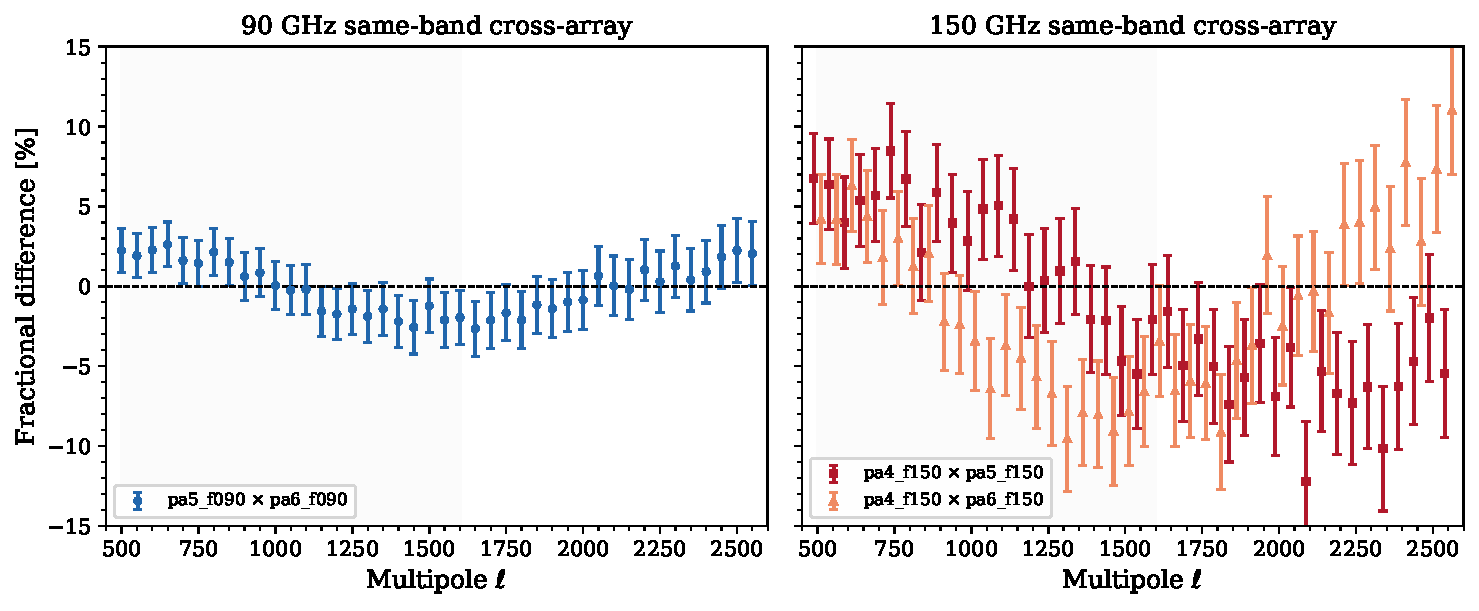
\includegraphics[width=\textwidth]{figures/fig1_sameband_crossarray.pdf}
\caption{Same-band cross-array fractional differences in split-cross TT spectra for the AA night maps.
\textit{Left:} 90\,GHz cross-array comparison (pa5\_f090 $\times$ pa6\_f090), showing tight agreement at the $\sim\!2\%$ level.
\textit{Right:} 150\,GHz cross-array comparisons, showing larger scatter at the $\sim\!7$--$9\%$ level.
The shaded region indicates the primary signal-dominated analysis range $500 \le \ell \le 1600$.
Error bars represent empirical split-cross scatter.}
\label{fig:sameband}
\end{figure*}

The strongest completed internal-consistency result is the beam-aware split-cross TT audit on AA night public maps.
In the signal-dominated range $500 \le \ell \le 1600$, same-band cross-array agreement at 90\,GHz is comparatively tight: pa5\_f090 versus pa6\_f090 yields a mean absolute fractional difference of $1.94\%$ and an rms fractional difference of $2.24\%$.
At 150\,GHz the same-band comparisons are broader: pa4\_f150 versus pa5\_f150 gives $7.28\%$ (mean absolute) and $9.14\%$ (rms), while pa4\_f150 versus pa6\_f150 gives $7.49\%$ and $9.17\%$, respectively.
These results are shown in Fig.~\ref{fig:sameband}.

\subsection{Cross-Frequency Consistency}\label{sec:crossfreq}

\begin{figure*}[t]
\centering
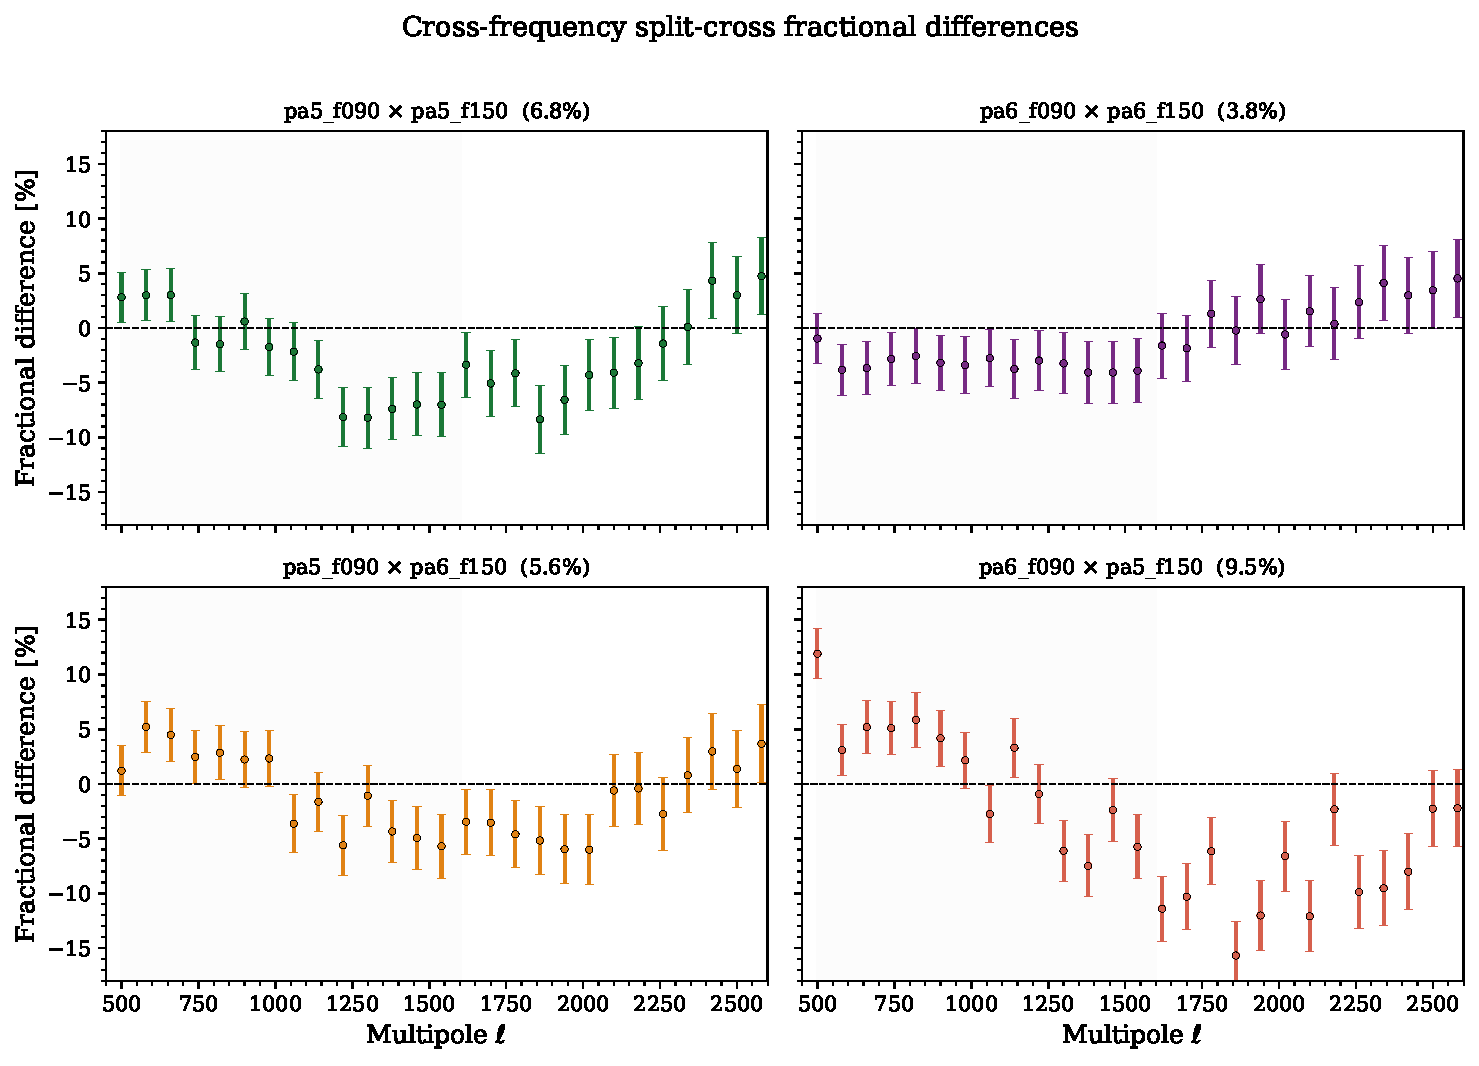
\includegraphics[width=\textwidth]{figures/fig2_crossfreq.pdf}
\caption{Cross-frequency split-cross fractional differences for four 90$\times$150\,GHz array combinations, shown in individual panels for clarity.
The mean absolute fractional difference ranges from $3.84\%$ (pa6\_f090 $\times$ pa6\_f150) to $9.47\%$ (pa6\_f090 $\times$ pa5\_f150) over $500 \le \ell \le 1600$.
These larger residuals are consistent with expectations from effective-frequency mismatch and foreground-weighting differences.
The shaded region indicates the primary analysis range.}
\label{fig:crossfreq}
\end{figure*}

Cross-frequency comparisons show larger residuals, as summarized in Table~\ref{tab:crossfreq} and Fig.~\ref{fig:crossfreq}.
The mean absolute fractional differences range from $3.84\%$ (pa6\_f090 $\times$ pa6\_f150) to $9.47\%$ (pa6\_f090 $\times$ pa5\_f150).
We interpret these few-to-$10\%$ residuals conservatively: they are consistent with the expectation that cross-frequency comparisons are intrinsically more sensitive to effective-frequency mismatch and foreground color differences than same-band checks.

\begin{table}[t]
\centering
\caption{Cross-frequency fractional differences for 90$\times$150\,GHz array pairs in the range $500 \le \ell \le 1600$.}
\label{tab:crossfreq}
\begin{tabular}{lcc}
\toprule
Channel pair & $\langle|\Delta C_\ell/C_\ell|\rangle$ [\%] & rms [\%] \\
\midrule
pa5\_f090 $\times$ pa5\_f150 & 6.80 & --- \\
pa6\_f090 $\times$ pa6\_f150 & 3.84 & --- \\
pa5\_f090 $\times$ pa6\_f150 & 5.59 & --- \\
pa6\_f090 $\times$ pa5\_f150 & 9.47 & --- \\
\bottomrule
\end{tabular}
\end{table}

\subsection{Within-Channel Split-Cross Stability}\label{sec:within}

\begin{figure}[t]
\centering
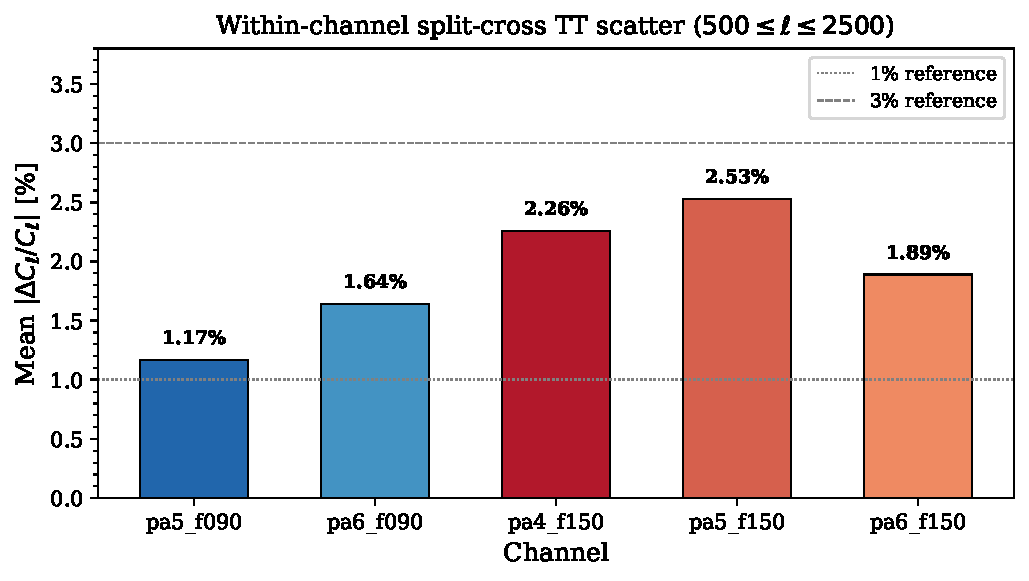
\includegraphics[width=\columnwidth]{figures/fig3_splitcross_scatter.pdf}
\caption{Mean absolute within-channel split-cross fractional scatter for each detector array over $500 \le \ell \le 2500$.
All channels show stability at the $1$--$3\%$ level, with pa5\_f090 exhibiting the tightest scatter ($1.17\%$).}
\label{fig:splitcross}
\end{figure}

A within-channel split-stability audit over $500 \le \ell \le 2500$ found mean absolute split-cross fractional scatter of $1.17\%$ for pa5\_f090, $1.64\%$ for pa6\_f090, $2.26\%$ for pa4\_f150, $2.53\%$ for pa5\_f150, and $1.89\%$ for pa6\_f150 (Fig.~\ref{fig:splitcross}).
This supports a provisional statement that same-channel split-cross TT stability is at the $1$--$3\%$ level in the signal-dominated regime.

\subsection{Day/Night and Cross-Array Residuals}\label{sec:daynight}

\begin{figure*}[t]
\centering
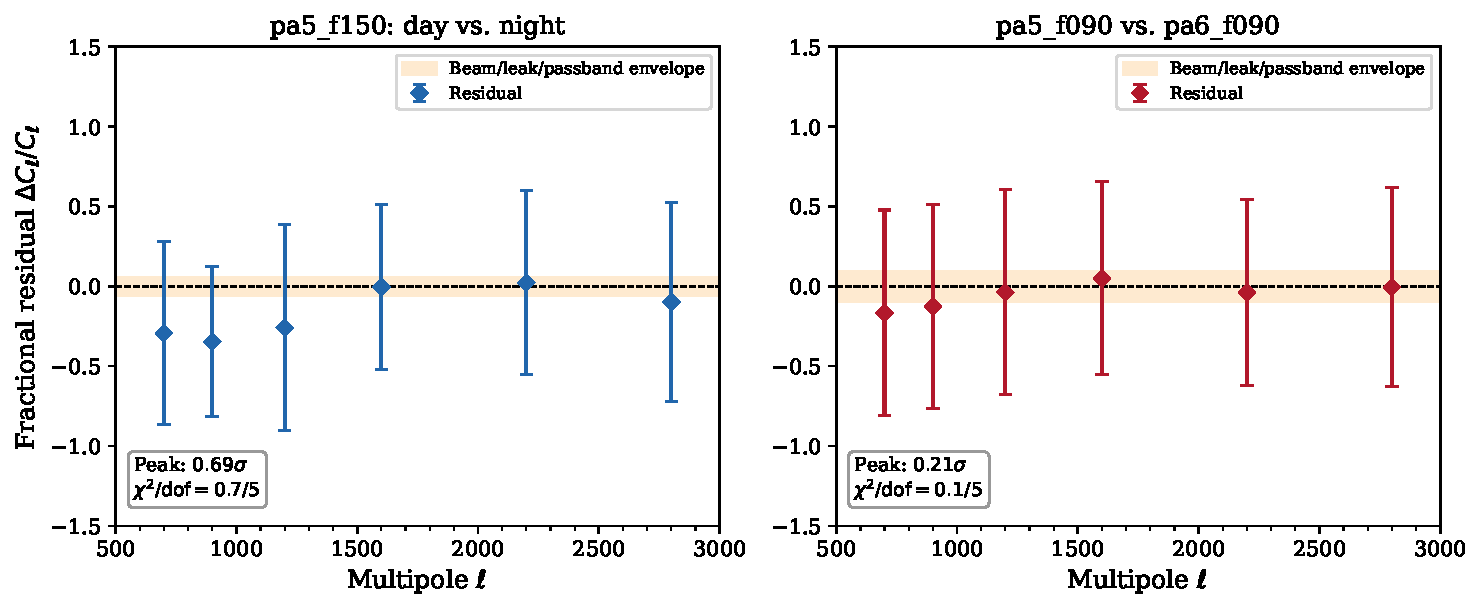
\includegraphics[width=\textwidth]{figures/fig4_residuals_envelopes.pdf}
\caption{Characterization of residual curves against expectation envelopes from released beam, leakage, and passband products.
\textit{Left:} pa5\_f150 day versus night comparison, with peak residual at $\ell \simeq 900$ reaching only $0.69\sigma$ significance.
\textit{Right:} pa5\_f090 versus pa6\_f090 cross-array comparison, with peak significance of $0.21\sigma$.
Orange bands show the simple beam/leak/passband expectation envelope; error bars represent empirical split-cross scatter.
In both cases, residuals exceed the expectation envelope but are not statistically significant.}
\label{fig:residuals}
\end{figure*}

The complementary characterization analysis produced two compact diagnostics over $600 \le \ell \le 2800$ (Fig.~\ref{fig:residuals}).
For pa5\_f150 day versus night, the peak fractional residual is $-0.382$ at $\ell \simeq 900$, while the beam/leak/passband expectation envelope is $0.055$ and the empirical split-cross scatter is $0.557$.
The resulting peak significance is $0.69\sigma$, with $\chi^2/\mathrm{dof} = 0.7/5$.
For the cross-array comparison pa5\_f090 versus pa6\_f090, the peak residual is $-0.134$ at $\ell \simeq 700$, for a peak significance of $0.21\sigma$ and $\chi^2/\mathrm{dof} = 0.1/5$.
In both cases, residual curves exceed the simple expectation bands but are not statistically significant once split-cross scatter is used as the uncertainty scale.

\subsection{Beam-Split Benchmarks}\label{sec:beamsplit}

\begin{figure}[t]
\centering
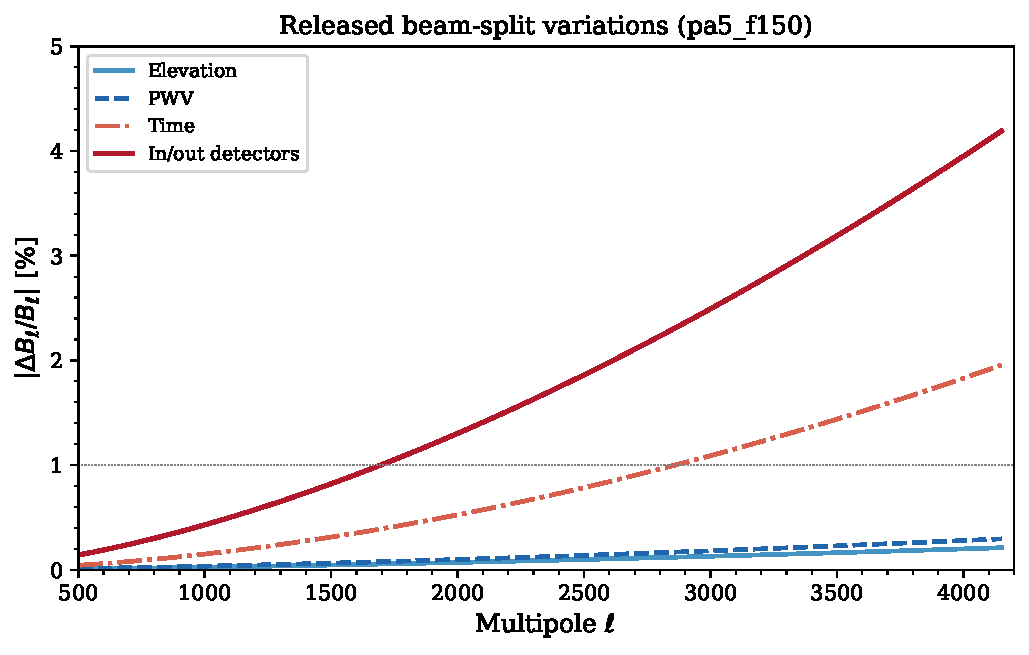
\includegraphics[width=\columnwidth]{figures/fig5_beam_splits.pdf}
\caption{Released beam-split variations for pa5\_f150 as a function of multipole.
Elevation and PWV splits produce sub-percent beam variations below $\ell < 4000$.
Time-split variations reach $\sim\!1.8\%$ in $B_\ell$ by $\ell = 4000$, while in/out detector splits are the dominant source at $\sim\!4\%$ in $B_\ell$ ($\sim\!8\%$ in power).}
\label{fig:beamsplits}
\end{figure}

Beam-split benchmarks provide context for interpreting the observed residuals.
For pa5\_f150, released elevation and PWV split-beam variations remain below $\sim\!0.2\%$--$0.3\%$ in $B_\ell$ for $\ell < 4000$, corresponding to sub-percent power-level effects (Fig.~\ref{fig:beamsplits}).
Time-split beam shape differences are larger after renormalization, reaching $\sim\!1.83\%$ in beam ($\sim\!3.67\%$ in power) by $\ell = 4000$.
In/out detector beam shape differences are the dominant released beam-split variation, reaching $\sim\!3.95\%$ in $B_\ell$ ($\sim\!7.91\%$ in power) by $\ell = 4000$.
These benchmarks suggest that released beam variations can plausibly contribute at the few-percent level in power at high $\ell$, but are not by themselves a sufficient explanation for every residual seen in simplified public-map comparisons.

\subsection{Source-Free versus Standard Maps}\label{sec:srcfree}

For the source-free versus standard map comparison, the key result is methodological: the benchmark should be performed channel-by-channel using only split-cross TT spectra, a common beam, and identical masks.
In this framework, the expected behavior is close agreement at low and intermediate multipoles, with differences emerging toward higher $\ell$ where point-source subtraction affects TT power.
We treat this as a transfer-impact validation axis rather than a calibration test, since source subtraction changes the sky content by design.

%----------------------------------------------------------------------
\section{Discussion}\label{sec:discussion}
%----------------------------------------------------------------------

\begin{figure}[t]
\centering
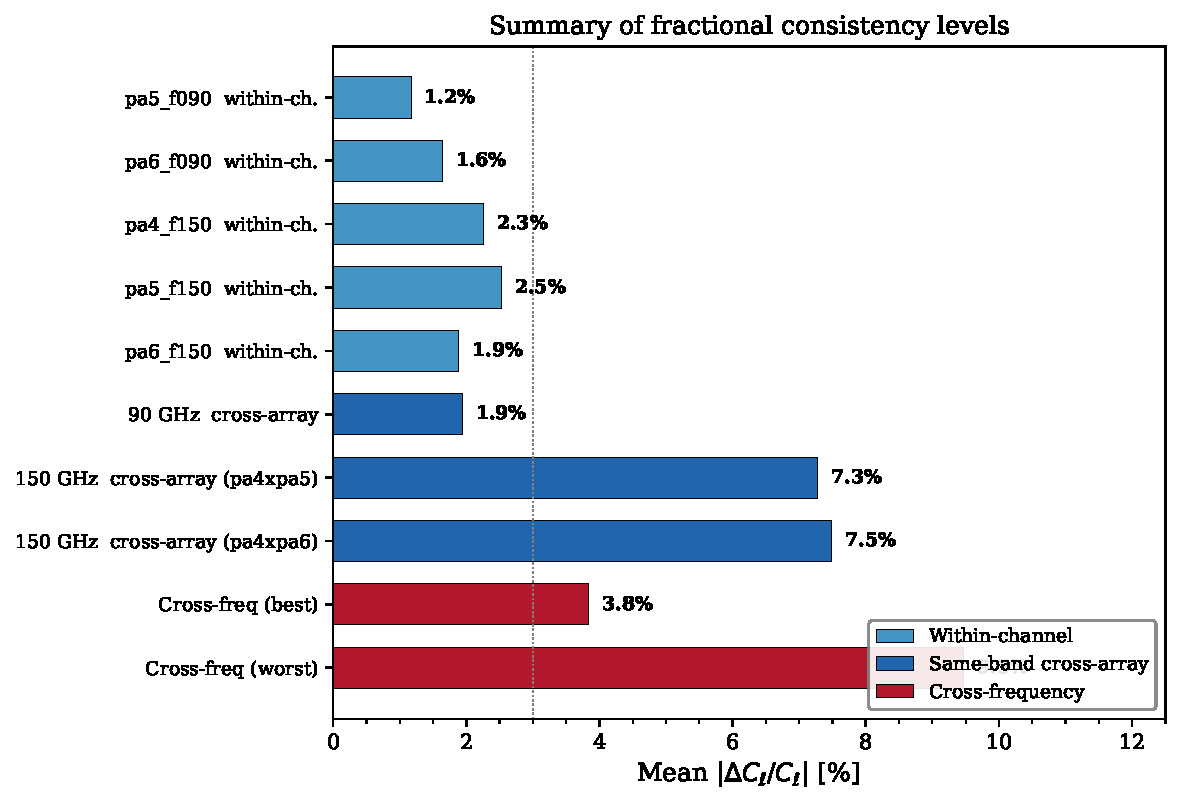
\includegraphics[width=\columnwidth]{figures/fig6_summary.pdf}
\caption{Summary of fractional consistency levels across all completed checks.
Within-channel split-cross scatter (blue) is at the $1$--$3\%$ level.
Same-band cross-array differences (dark blue) are $\sim\!2\%$ at 90\,GHz but $\sim\!7$--$9\%$ at 150\,GHz.
Cross-frequency residuals (red) range from $\sim\!4\%$ to $\sim\!10\%$.
The vertical dotted line marks the $3\%$ reference level.}
\label{fig:summary}
\end{figure}

The principal finding of these completed checks is a coherent hierarchy of consistency levels, summarized in Fig.~\ref{fig:summary}.
Same-channel split stability is typically at the $1$--$3\%$ level in the signal-dominated TT regime.
Same-band cross-array agreement is strongest at 90\,GHz and looser at 150\,GHz.
Cross-frequency residuals are larger still, plausibly attributable in part to effective-frequency mismatch and foreground-color differences.

This hierarchy has practical implications for users of the public release.
Same-channel split-cross tests are the cleanest released-product benchmark because they avoid auto-spectrum noise bias, minimize spectral mismatch, and are directly sensitive to internal processing stability.
Same-band cross-array tests are informative but more demanding, particularly once beam differences and passband mismatch are included.
Cross-frequency tests serve as broad sanity checks but should not be overinterpreted without explicit foreground modeling.

The source-free versus standard comparison occupies a different conceptual category.
Since the map pair is not expected to be identical---one product has had detected point sources subtracted---the correct validation question is whether the observed TT differences are bounded, scale-dependent in the expected sense, and stable under the same split-cross procedure used elsewhere.

A second important lesson is procedural: the common-beam repair changed the evidentiary value of the consistency tests.
This underscores that executable benchmarks should precede broad claims.
In practice, the minimal benchmark that best anchors this analysis is a one-channel split-cross TT comparison between standard and source-free maps using explicit data paths, a single nominal beam, and reproducible outputs.

We acknowledge several limitations.
The present analysis uses flat-sky FFT pseudo-$C_\ell$ estimates on cropped patches with approximate mask normalization.
It does not include a full mode-coupling matrix, transfer-function correction, or collaboration-grade covariance.
Beam uncertainty propagation is represented only indirectly through released beam-split envelopes.
Null-map replication in the same framework remains incomplete, and robustness to alternate patch and mask choices has not been established at full publication depth.

%----------------------------------------------------------------------
\section{Conclusions}\label{sec:conclusions}
%----------------------------------------------------------------------

We have presented a released-product validation analysis of ACT DR6 temperature maps using beam-aware split-cross pseudo-$C_\ell$ estimators built entirely from public data products.
Our main conclusions are:

\begin{enumerate}
\item \textbf{Beam-aware common-beam handling is essential.} Correcting the harmonization step in harmonic space with proper $a_{\ell m}$ indexing substantially improved the interpretability of split-cross comparisons.

\item \textbf{Within-channel TT split-cross stability is at the $1$--$3\%$ level} in the signal-dominated multipole range for the public AA night maps. This is the cleanest internal consistency result, relying only on independent split-crosses within a single channel.

\item \textbf{Same-band cross-array agreement is tighter at 90\,GHz ($\sim\!2\%$) than at 150\,GHz ($\sim\!7$--$9\%$),} while cross-frequency residuals are at the few-to-$10\%$ level. The latter are plausibly attributable to passband-driven effective-frequency mismatch and foreground-color sensitivity, not calibration failure.

\item \textbf{Residual curves can exceed simple expectation envelopes} derived from released beam, leakage, and passband products, but they are not statistically significant relative to empirical split-cross scatter.
\end{enumerate}

These results demonstrate that public ACT DR6 temperature products pass a useful set of beam-aware split-cross validation tests at the level expected for released-product characterization.
They provide valuable diagnostics for users of the public release but should be understood as audit-level validation, not as substitutes for the official ACT DR6 spectrum~\cite{Louis2025} or likelihood pipelines.

Natural extensions include null-map replication, explicit source-free versus standard summary tables across channels, robustness tests with alternate masks and patches, and promotion of the strongest diagnostics to a mode-coupling-corrected pseudo-$C_\ell$ framework.

%----------------------------------------------------------------------
\begin{acknowledgments}
This analysis was produced by the CosmoEvolve autonomous research lab using publicly available ACT DR6.02 data products.
We acknowledge the use of the \texttt{pixell} software package for map manipulation and harmonic-space operations.
\end{acknowledgments}

\bibliography{references}

\end{document}
